%!TEX root = paper.tex
%%%%%%%%%%%%%%%%%%%%%%%%%%%%%%%%%%%%%%%%%%%%%%%%%%%%%%%%%%%%%%%%%%%%%%%%%%%%%%%
\section{Models}


%%%%%%%%%%%%%%%%%%%%%%%%%%%%%%%%%%%%%%%%%%%%%%%%%%%%%%%%%%%%%%%%%%%%%%%%%%%%%%%
\subsection{Cost Model}


\todo[inline]{Vermutlich lassen wir das Extensive Model vorerst sein, was bedeuten wuerde, dass wir bei Efficiency einsteigen koennten...}

$c$: cost
$t$: time
$d$: demand
$p$: price
$u$: use(?)
$i$: investment(?)

%%%%%%%%%%%%
\subsubsection{CAPEX}

Regionale Data Center => SERVER HARDWARE? (siehe unterhalb?)

Gaming Server (GPU-Enabled) => vermutlich ebenso aggregiert enthalten unten?

Entwicklungskosten für Software-Plattform(?) => noch nicht enthalten? Wie hoch sind die Anpassungskosten?

CAPEX in our case is a dimensioning problem.

CAPEX are typically used in the sense of depreciation costs. We have to define the runtime of hardware and calculate the cost per user and year to understand whether it is profitable on a per contract basis later on.

Probably we have to fill this model on a per regional data center perspective??

\begin{align*}
u_{peak} = Users \cdot peak\_load\_factor \\
d_{peak\_resource} = peak\_use \cdot d_{average\_resource} \\
d_{peak\_quality} = peak\_use \cdot overprovisioning \\
c_{infrastructure} = d_{peak\_quality} \cdot i_{resource\_unit}
\end{align*}

$game\_adaptation\_costs = XXXXX$ => meine Vermutung: Integration über Prozentsatz am Licensing in OPEX leichter, da schätzbar?

Depreciation times in Germany for mainframes: 7 years [Quelle noch ausstaendig.. Gesetz?]
fm: I would argue that gaming servers lose their value much more quickly than regular servers: you won't be able to run a current game on a 7-year old machine in a reasonable quality. At least the number of games will be very limited, reducing their value. 
You would probably need to mix in new hardware every 2-3 years.

Ok, but what's the full cycle to completely swap the hardware or double it up? If it is 5-6 years, then the depreciation time is 5-6 years. If it is lower than that, we go lower etc. etc. It is fair to argue 7 years is too much, but the server might have a 7-year value if it is generic hardware that is just used for games. Otherwise the value has decreased to 0 in the 5-6 years range. I need to do some research here :D

\begin{align*}
CAPEX_{year} = \frac{c_{infrastructure}}{7} \\
CAPEX_{contract} = \frac{CAPEX_{year}}{users}
\end{align*}
Note: Users are kept static for the one-shot analysis. 


%%%%%%%%%%%%
\subsubsection{OPEX}

OPEX consists of several components: Network traffic generates costs (interconnection fees and/or wholesale Internet access fees); energy; maintenance (replacement units and cost to replace and monitor things); licensing (probably it's a per year fee rather than a ``purchase'' => shift to CAPEX otherwise)

\begin{align*}
t_{use} = users \cdot t_{avg\_per\_year} \\
c_{energy} = t_{use} \cdot d_{avg\_energy} \cdot p_{energy\_unit} \\
c_{network} = t_{use} \cdot d_{avg\_network\_res} \cdot p_{network\_unit} \\
c_{maintenance} = t_{use} \cdot failure\_propability \cdot c_{failure} \\
c_{licensing} = t_{use} \cdot p_{license\_per\_t_{use}} \\
OPEX_{year} = c_{energy} + c_{network} + c_{maintenance} + c_{licensing} \\
OPEX_{contract} = \frac{OPEX_{year}}{users}
\end{align*}

failure costs: (personnel; replacement\_units; etc.) 

%%%%%%%%%%%%
\subsubsection{CUSTOMER COSTS / CONSUMER RATIONALE}

The customer pays the revenue (see below) + hardware costs. Substitutes (like Steam or classical console games) can be compared on this basis or on the revenue side to understand how much one can price for it.

200(++) for hardware but probably we can use the depreciation time of 4 years here. 
=> Hardware costs: $ \frac{\SI{200}{\EUR}}{5}  = \SI{40}{\EUR}$

\begin{align}
End\_customer\_cost\_per\_year = R/users + 40
\end{align}

Now compare to alternatives. An alternative i is dominated by j if $End\_customer\_cost\_per\_year ** i > End\_customer\_cost\_per\_year ** j$

Alternative products are: Console games, PC games, steam, etc.

If no feasible revenue model can be found to both generate profit and to satisfy the customer rationale, the model is unsuccessful and does not stand the competition with substitutes.



%%%%%%%%%%%%%%%%%%%%%%%%%%%%%%%%%%%%%%%%%%%%%%%%%%%%%%%%%%%%%%%%%%%%%%%%%%%%%%%
\subsection{Revenue Model}

\begin{align*}
p_{year} &= 12 \cdot p_{month} \\
p &= \frac{p_{year}}{avg\_time\_per\_year} \\
R &= p  \cdot t_{usage} \text{ OR } p_{year} \cdot users
\end{align*}


%%%%%%%%%%%%%%%%%%%%%%%%%%%%%%%%%%%%%%%%%%%%%%%%%%%%%%%%%%%%%%%%%%%%%%%%%%%%%%%
\subsection{Profit Model}

\begin{align*}
M(P & =R-C)E \\
C &= CAPEX\_per\_contract + OPEX\_per\_contract \\
R &= \text{see above...}
\end{align*}

$M / E$ are external factors, which are probably not supported by equations. Let's see later.


\subsection{Computational Efficiency}

Based on the collected consumer price figures of Section XXX, this section will elaborate on the required computational efficiency, i.e., cost per hosted subscriber, in order to successfully establish cloud gaming approaches on the market. Due to the limited available data, this investigation will follow a one data center assumption. Due to the demands of cloud gaming to serve both high performance and low latency, regional data centers will play a dominant role in the provider side cost modelling. 

\begin{figure}[!t]
	\centering
	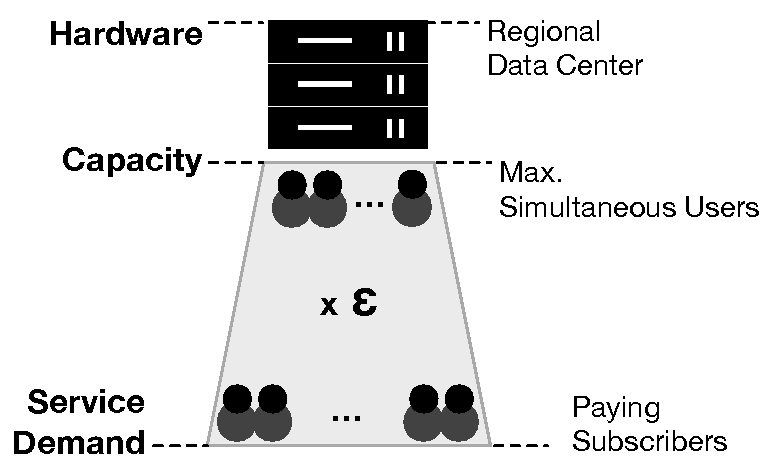
\includegraphics[width=0.65\columnwidth]{images/overbooking_datacenter.pdf}
	\caption{Overbooking of available computational capacity.}
\label{fig:overbooking_datacenter}
\end{figure}

The computational efficiency further considers the maximum overbooking rate $\epsilon \geq 1$, where $\epsilon = 1$ refers to no overbooking. $\epsilon$ is calculated as ratio of the peak utilization $d_{peak}$ (number of peak time users) from the overall capacity $Cap$, 

\begin{equation}
	\epsilon = \frac{Cap}{d_{peak}} \quad ,
\end{equation}

where $Cap$ refers to the number of subscribed users that can be handled simultaneously by this data center. The maximum number of subscribers $d$ (maximum service demand) is, thus, given by

\begin{equation}
	 d = Cap \cdot \epsilon \quad .
\end{equation}

The average monthly customer price $\bar{p}$ aggregates the monthly subscription fee and the customer's depreciation costs for the hardware investments on a four years investment duration. We further consider a minimum profit margin $m$ of $3 \%$, which is in line with the average figure for the global game industry\footnote{\url{http://www.polygon.com/2012/10/1/3439738/the-state-of-games-state-of-aaa}} and substantially below the cloud computing figures that can range up to $16.9\%$\footnote{\url{http://www.forbes.com/sites/georgeanders/2015/04/23/amazons-web-services-delight-16-9-margins-more-joy-ahead/\#73324aa64b4e}} and potentially even higher\footnote{\url{http://www.bloomberg.com/news/articles/2015-12-02/microsoft-should-disclose-cloud-revenue-margins-ballmer-says}}.

%Global Games statistics / billion revenues 2012-2016: http://newzoo.com/infographics/global-games-market-report-infographics-2013/
% Game industry = 3%: http://www.polygon.com/2012/10/1/3439738/the-state-of-games-state-of-aaa
% Game industry in the past (2009 – average console game with margin of 40%): http://www.businessinsider.com/casual-gaming-profit-margins-near-90-2009-10?IR=T
% Profit margins in cloud computing:
%	Amazon 16.9% (2015): http://www.forbes.com/sites/georgeanders/2015/04/23/amazons-web-services-delight-16-9-margins-more-joy-ahead/#73324aa64b4e
% 	Microsoft 44% (2015) -- questionable: http://www.bloomberg.com/news/articles/2015-12-02/microsoft-should-disclose-cloud-revenue-margins-ballmer-says

\begin{align} \label{eq:computational_efficiency}
	\frac{\epsilon \cdot Cap \cdot \bar{p}}{Cap} :=& \underbrace{\frac{C_{cap}}{Cap}}_{C_{u}} \cdot m =\\
	=\frac{C_{cap}}{Cap} :=& \epsilon \cdot \bar{p}
\end{align}

When treating the costs of the regional data center as blackbox (operational and capital costs for the data center, and required game licensing fees), the analysis can concentrate on the required capacity and licensing cost $C_{u}$ per connected user $u$.

%\begin{equation}
%	ce = \frac{C_{cap}}{Cap} \quad .
%\end{equation}

For obtaining the required minimum margin $m$, the capacity and licensing cost per user $ce$ needs to be below XXXXXXXX Euro.

\todo[inline]{NOW LET'S ADD THE DATA}

The overbooking ratio $\epsilon$ could also be increased by models fostering the off-peak usage, e.g., off-peak subscriptions that only allow access to the platform outside peak hours. When considering a substantial increase of the $\epsilon$ to $1.5$---the realistic maximum when considering the high peak time centricity of the gaming use case---, we obtain a substantially lowered $C_{u}$ requirement of 

\todo[inline]{ADD DATA}

Due to the requirement of using special hardware that is focused on the gaming use case, hardware sharing with other cloud applications seems unrealistic. Thus, we can characterise that the successful will have a maximum $C_{u}$ in the following bounds:

\todo[inline]{XXX}

This maximum does not consider that the operator may not be able to fully utilize the available capacity or may not hold the optimal game licenses at all times. Thus, in practice, the required hardware costs per subscriber have to be lower than $C_{u}$ .

\todo[inline]{NOW LET'S INTERPRET IF THAT SOUNDS LIKE A HARD THING TO DO OR NOT. AND THERE WE GO.}



